\documentclass[a4paper, 12pt]{article}

\usepackage{url}
\usepackage{graphicx}
\usepackage{caption}
\usepackage[section]{placeins}
\usepackage{fixltx2e}
\usepackage[page]{appendix}

\usepackage{amsmath}
\usepackage{cleveref}

%for code(MATLAB in particular)
\usepackage{listings}
\usepackage{color} %red, green, blue, yellow, cyan, magenta, black, white
\definecolor{mygreen}{RGB}{28,172,0} % color values Red, Green, Blue
\definecolor{mylilas}{RGB}{170,55,241}

% Default fixed font does not support bold face
\DeclareFixedFont{\ttb}{T1}{txtt}{bx}{n}{12} % for bold
\DeclareFixedFont{\ttm}{T1}{txtt}{m}{n}{12}  % for normal

% Custom colors
\usepackage{color}
\definecolor{deepblue}{rgb}{0,0,0.5}
\definecolor{deepred}{rgb}{0.6,0,0}
\definecolor{deepgreen}{rgb}{0,0.5,0}

\lstset{
    language=Matlab,%
    %basicstyle=\color{red},
    breaklines=true,%
    morekeywords={matlab2tikz},
    keywordstyle=\color{blue},%
    morekeywords=[2]{1}, keywordstyle=[2]{\color{black}},
    identifierstyle=\color{black},%
    stringstyle=\color{mylilas},
    commentstyle=\color{mygreen},%
    showstringspaces=false,%without this there will be a symbol in the places where there is a space
    numbers=left,%
    numberstyle={\tiny \color{black}},% size of the numbers
    numbersep=9pt, % this defines how far the numbers are from the text
    emph=[1]{for,end,break},emphstyle=[1]\color{red}, %some words to emphasise
    %emph=[2]{word1,word2}, emphstyle=[2]{style},
}


\graphicspath{{./pictures/}}

\title{ECEN321 - Lab 4 \\
    Hypothesis Testing
}
\author{Joshua Benfell - 300433229}

\begin{document}
    \maketitle
    
    \section{Introduction}
        In this report a hypothesis test will be performed and analysed. The null hypothesis is that realisations of a poisson generated random variable is actually from a poisson distribution. This will be tested using a $\chi^2$ test. Consequently the alternate hypothesis is that the poisson random variable is not from a poisson distribution.

    \section{Method}
        To test this hypothesis, $M = 100$ inter-arrivals will be generated from a Poisson random variable. This will be done by transforming a uniform random variable into a poisson random variable. To do this we take the negtaive log of the uniform random variable and divide it by the poisson parameter $\lambda = 3$. From here, the cumulative sum is taken of the inter arrival times to find the times when arrivals happen. 
        \par
        Now that an experimental data from a poisson random variable has been set up we can calculated the number of observed events. We take the sum of all the arrivals times that are less than time $t=5$. This gives us the number of events that happen in less that the time period specified. This can then be plotted against the range of events that can happen $K = [0 ... t \times \lambda \times 2]$ which gives us an observed pdf of how many events happened in time $t$.
        \par
        An expected distribution needs to be constructed for comparison with the $\chi^2$ test. The poisson distribution PDF \cref{eq:poisson pdf} is used, with the above stated parameters, and scaled by the number of trials $N$ to align it with the observed values and get a count of the expected events in time $t$.

        \begin{equation}
            \label{eq:poisson pdf}
            p_{K(t)}(k) = \frac{e^{-\lambda t}(\lambda t)^k}{k!}
        \end{equation}
        \begin{equation}
            \label{eq:chi2}
            \Sigma \frac{(Observed - Expected)^2}{Expected}
        \end{equation}

        To perform a $\chi^2$ test, all the bins of the datasets need to have at least 5 events in them. We pile all values less than 5 into one bin on either side to achieve this. From here the $\chi^2$ value is calculated \cref{eq:chi2} and compared to the critical value found from a lookup table related to the confidence level ($0.01$) and the degrees of freedom $\nu$. If the $\chi^2$ value is significantly larger than the critical value, then the null hypothesis can be rejected.


        \section{Results}
            \begin{figure}[!h]
                \centering
                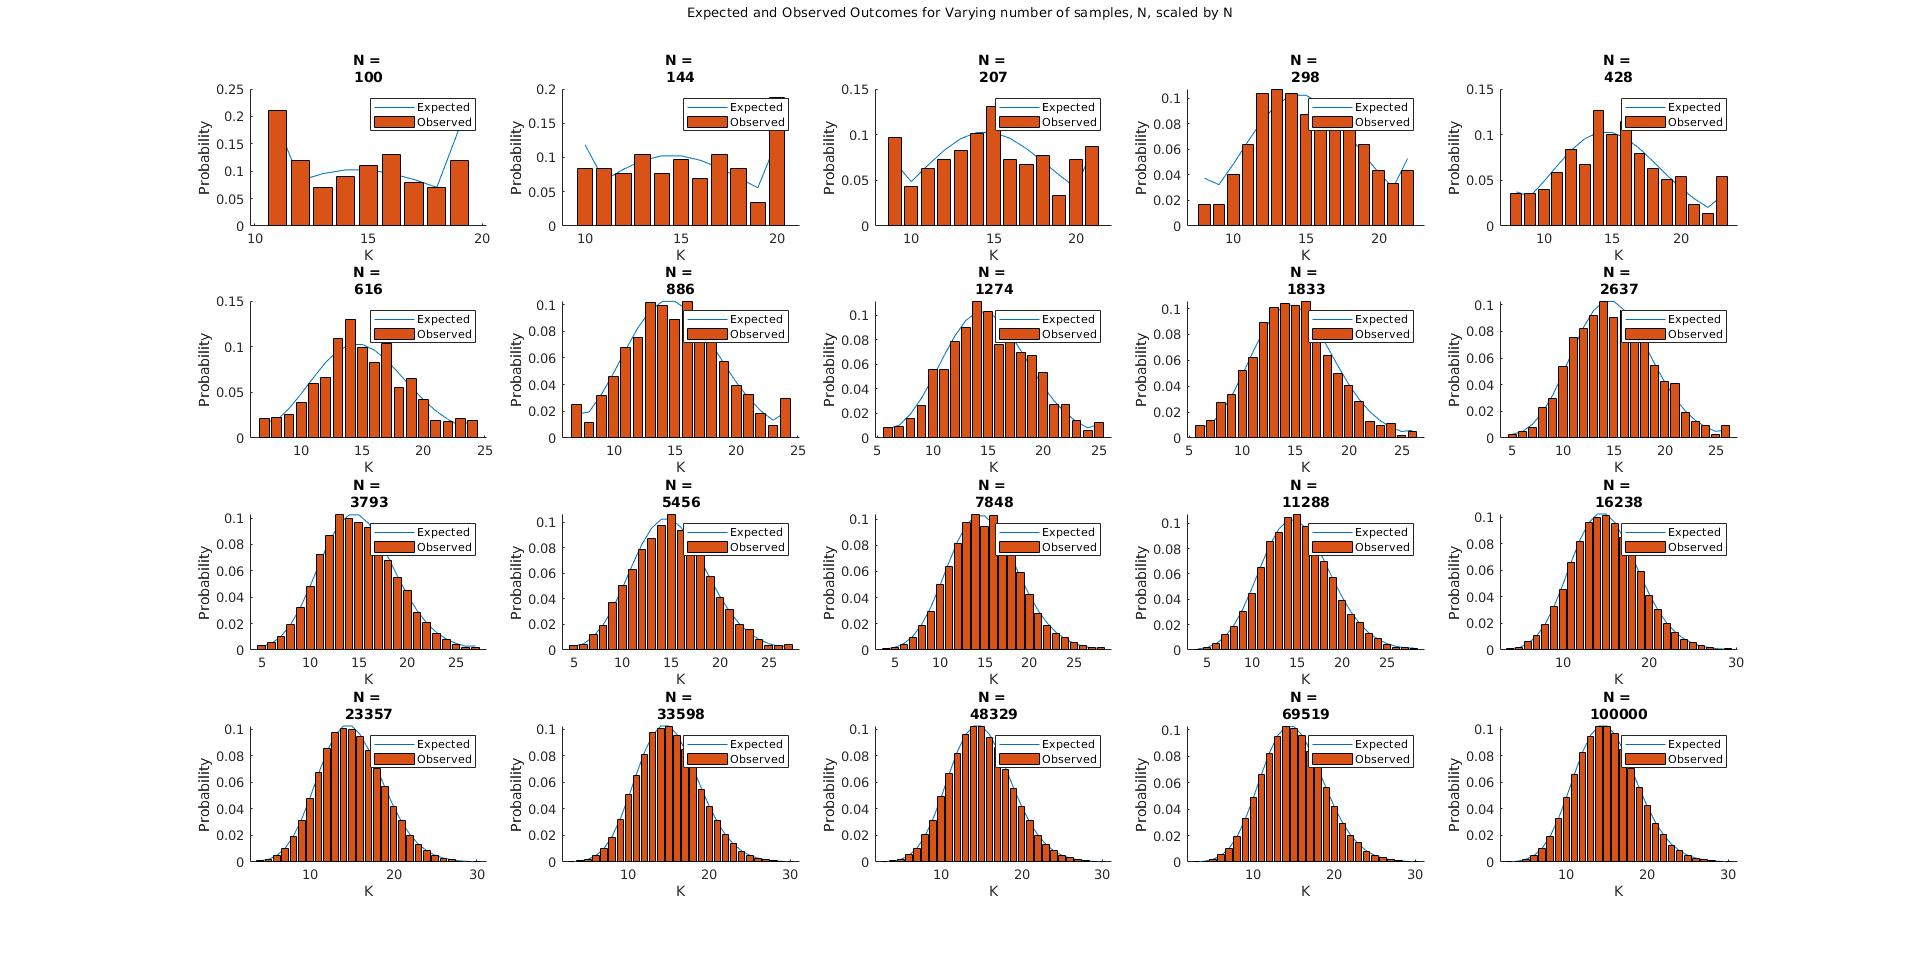
\includegraphics[width=\textwidth]{observerdVsExpected.jpg}
                \caption{Plots of expected and observed outcomes for different values of N}
                \label{fig:plot}
            \end{figure}
            \begin{table}
                \centering
                \begin{tabular}{r|r|r}
                    \textbf{N} & \textbf{$\chi^2$ Value} & \textbf{Critical Value} \\
                    \hline
                    100 & 6.149282073 & 20.09023503 \\
                    144 & 11.05540555 & 23.20925116 \\
                    207 & 13.04708368 & 26.21696731 \\
                    298 & 13.12529465 & 29.14123774 \\
                    428 & 18.06504567 & 30.57791417 \\
                    616 & 22.74178331 & 33.40866361 \\
                    886 & 15.78066836 & 33.40866361 \\
                    1274 & 24.72741788 & 36.19086913 \\
                    1833 & 29.03443487 & 37.56623479 \\
                    2637 & 33.14307315 & 38.93217268 \\
                    3793 & 12.28919969 & 40.28936044 \\
                    5456 & 28.08687747 & 40.28936044 \\
                    7848 & 22.88582981 & 42.97982014 \\
                    11288 & 26.27790647 & 42.97982014 \\
                    16238 & 31.54759935 & 44.3141049 \\
                    23357 & 14.80776634 & 45.64168267 \\
                    33598 & 53.46831014 & 46.96294212 \\
                    48329 & 34.1201107 & 46.96294212 \\
                    69519 & 40.97674385 & 46.96294212 \\
                    100000 & 30.55728852 & 46.96294212 \\
                \end{tabular}
                \caption{Table of $\chi^2$ and critical values for different values of N}
                \label{tab:values}
            \end{table}
            \Cref{fig:plot} contains the expected and observed datasets for our trials of various sizes N. Visually we can see that the plots all line up pretty well. At low N values, the combination of the count of events being less than 5 has a significant effect, causing the sides to spike up more than the values beside it. This is reflected in the fact that the plots look more flat than they normally would, as seen at higher values of N.
            \par
            \Cref{tab:values} contains all the critical and $\chi^2$ values for each run of N trials. For almost all the values of N, the $\chi^2$ value is less than the critical value. The value that is greater than the critical value has failed the test. On reruns of the test, there would always be one or two cases where the $\chi^2$ value was larger than the critical value. 
            \par
            \begin{figure}[!h]
                \centering
                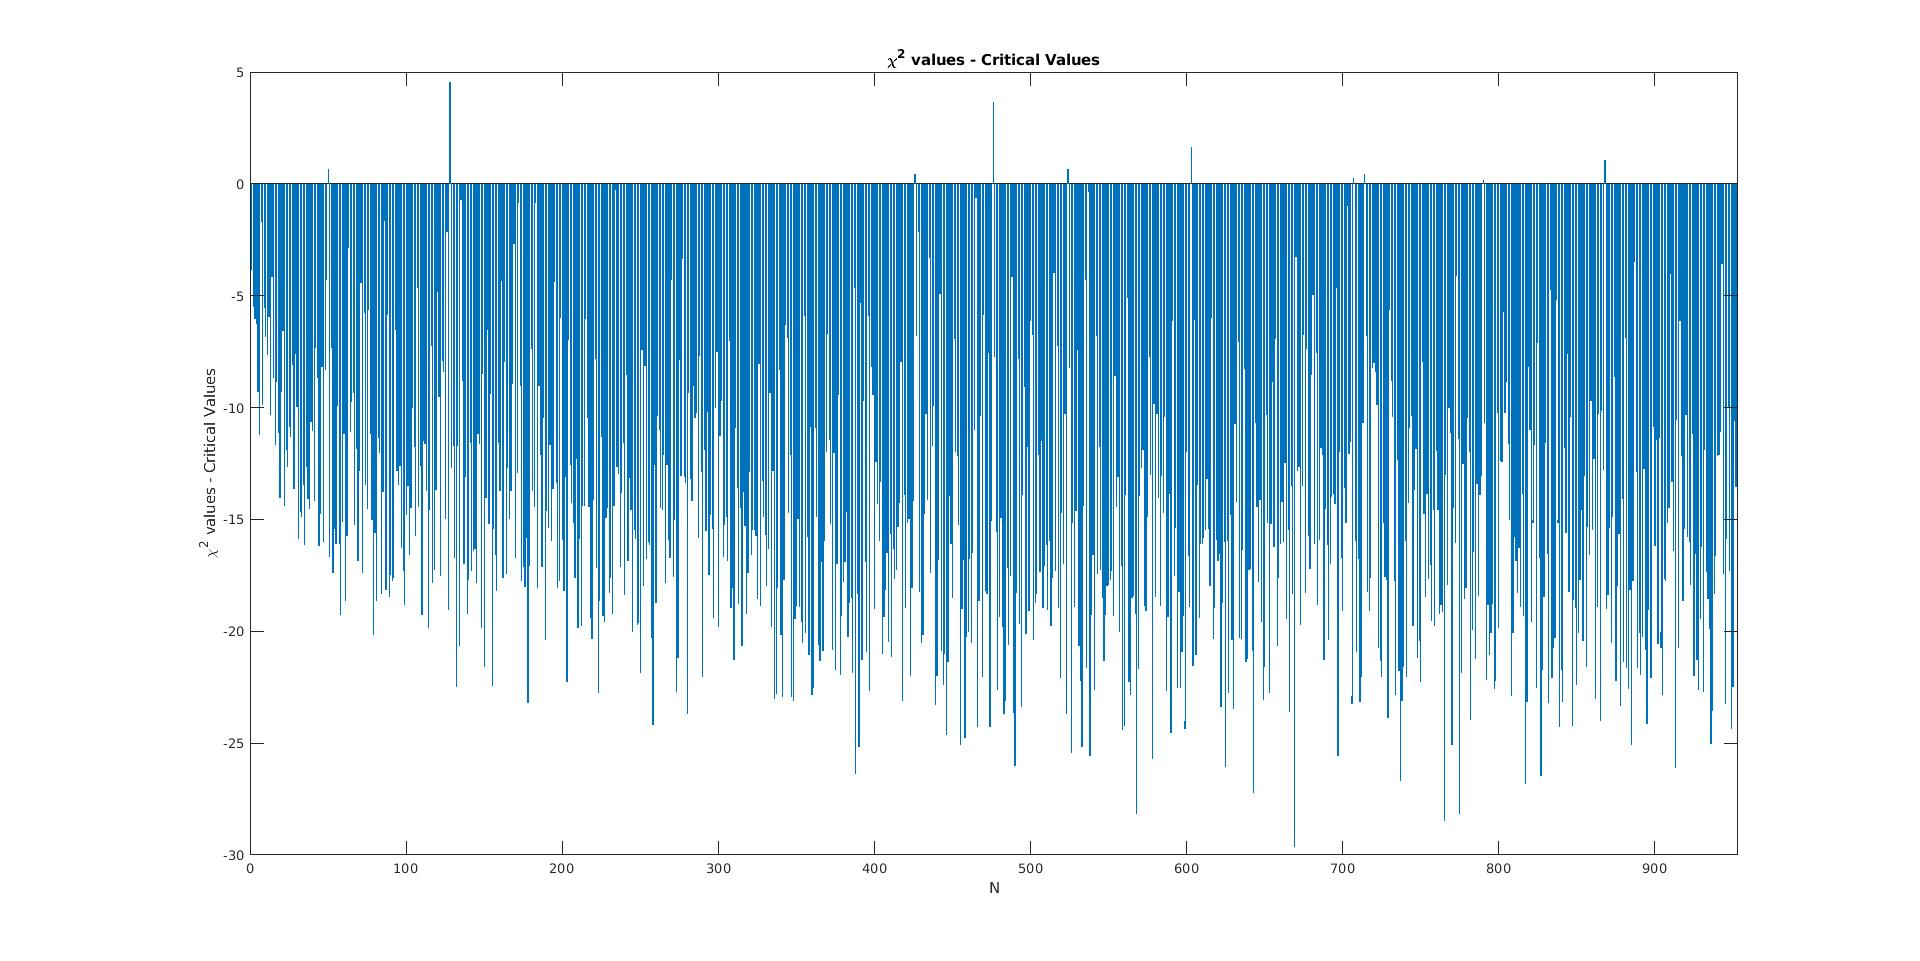
\includegraphics[width=\columnwidth]{failures.jpg}
                \caption{Positive values of $\chi^2 - critical$ are fails }
                \label{fig:fails}
            \end{figure}
            The minimum value of N we need to pass the null hypothesis is 49 as the variables are all from the poisson distribution, we are forcing them this way, and values below this don't provide enough samples to have all values more than 5, and would result in a single bar for both expected and observed outcomes. We can see an outcome in \cref{fig:fails} where not many cases do fail at 49 and above to 1000. In a test where you are unsure about which distribution they belong to would not have this as the case.
            \par
            From \cref{tab:values} it can be concluded that the null hypothesis of realisation of a poisson random variable belonging a poisson distribution is credible. This hypothesis can never be proven as all it takes is one case to not belong to the poisson distribution. Which it looks like we occasionally get with the $\chi^2$ test value being higher than the critical value. So most of the time it is possible to conclude that our realisations belong to a poisson distribution.
        
    \section{Conclusion}
        In this report we covered a hypothesis test on the null hypothesis, realisations of a poisson random variable belong to the poisson distribution and alternate hypothesis that they don't. We tested this hypothesis by using the $\chi^2$ test on a transformed uniform random variable. From performing this test many times for varying N realisations, it was found that this hypothesis is credible and holds true, but it occasionally may fail. It was also found that doing more than $\sim 33000$ tests leads to no increase in the critical value and therefore no further improvement in the test.

    % \Urlmuskip=0mu plus 1mu\relax
    % \bibliography{bibliography}
    % \bibliographystyle{IEEEtran}

    \begin{appendices}
        \section{MATLAB Code}
            \lstinputlisting{../lab4.m}
    \end{appendices}
\end{document}